\documentclass[uct_visualisation_thesis.tex]{subfiles}

W celu poprawnego działania aplikacji niezbędna jest efektywna komunikacja między jej komponentami. Niniejszy rozdział poświęcony jest opisowi procesu komunikacji komponentów, który jest odzwierciedleniem implementacji architektury programu.

\section{Struktura klas} \label{subsec:uml}
W celu poprawnego działania aplikacji niezbędna jest efektywna komunikacja między jej komponentami. Niniejszy rozdział poświęcony jest opisowi procesu komunikacji komponentów, który jest odzwierciedleniem implementacji architektury programu.

\begin{figure}[h!]
	\centering
	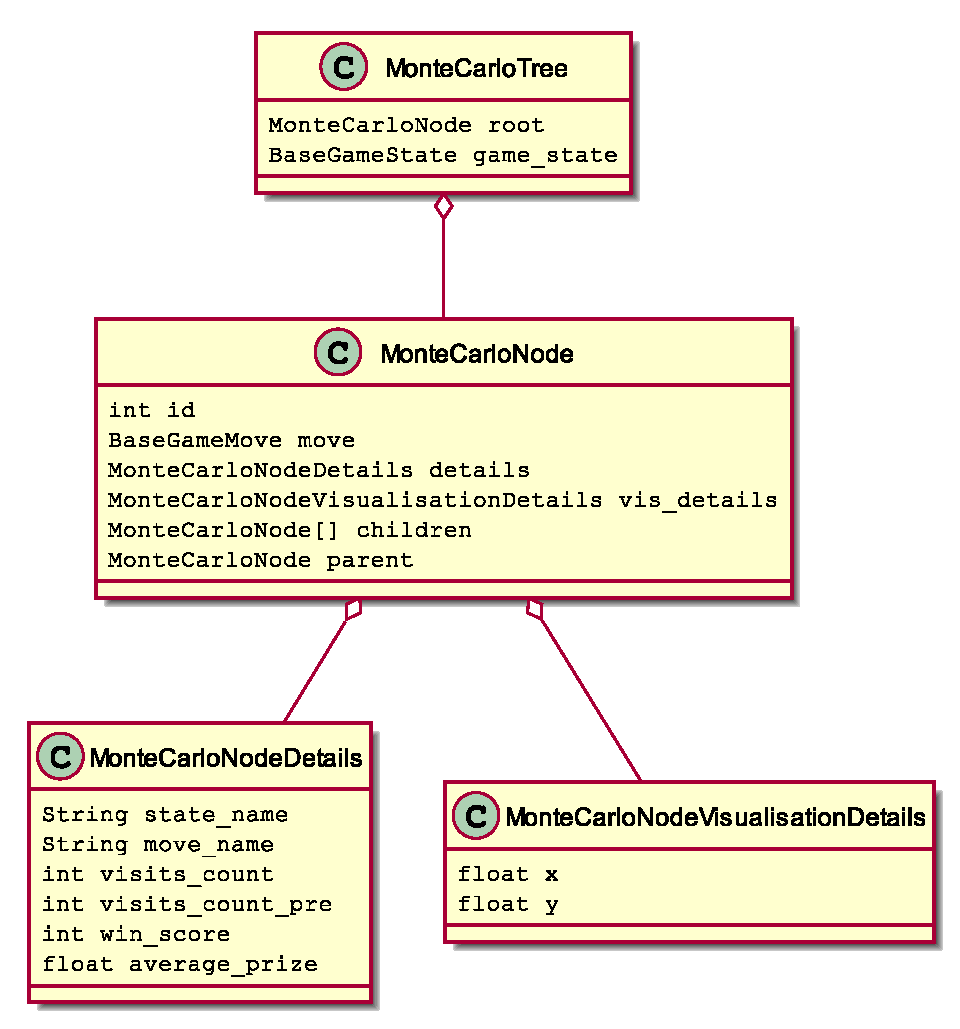
\includegraphics[width=0.5\linewidth]{umldiagram_node}
	\caption{Diagram UML klasy wierzchołka}
	\label{rys:umldiagram_node}
\end{figure}

Klasa \textit{MonteCarloNode}, zgodnie z Rysunkiem\footnote{Diagramy na Rysunkach \ref{rys:umldiagram_node}-\ref{rys:sequencevisualise} zostały wygenerowane z użyciem oprogramowania \textit{PlantUML} na licencji \textit{GNU General Public License}.} \ref{rys:umldiagram_node}, reprezentuje wierzchołek w drzewie, więc przechowuje referencje do swojego rodzica i wierzchołków potomnych, aby zachować rekurencyjną strukturę drzewa. Ponadto zawiera wszystkie informacje związane z przebiegiem algorytmu UCT w polu \textit{details} oraz algorytmu Walkera w polu \textit{vis\textunderscore details}. \\

Diagram ukazany na Rysunku \ref{rys:umldiagram_algorithm} ukazuje najistotniejsze klasy modułu \textit{Algorytm}. Metoda \textit{calculate\textunderscore next\textunderscore move} klasy \textit{MonteCarloTreeSearch} odpowiada za wykonanie kolejnych iteracji algorytmu. Algorytm zapisuje informacje o rozgrywanych playoutach w polach klasy \textit{MonteCarloNodeDetails} analizowanych wierzchołków. Ruch oraz stan analizowanej gry są opisane odpowiednio przez klasy \textit{GameMove} i \textit{GameState}. Implementacja metod tych klas daje możliwość łatwego rozszerzenia aplikacji o inne gry. Istotny z punktu widzenia konstrukcji drzewa jest stan rozgrywki, który opisują pola typu wyliczeniowego \textit{GamePhase}.

\begin{figure}[h!]
	\centering
	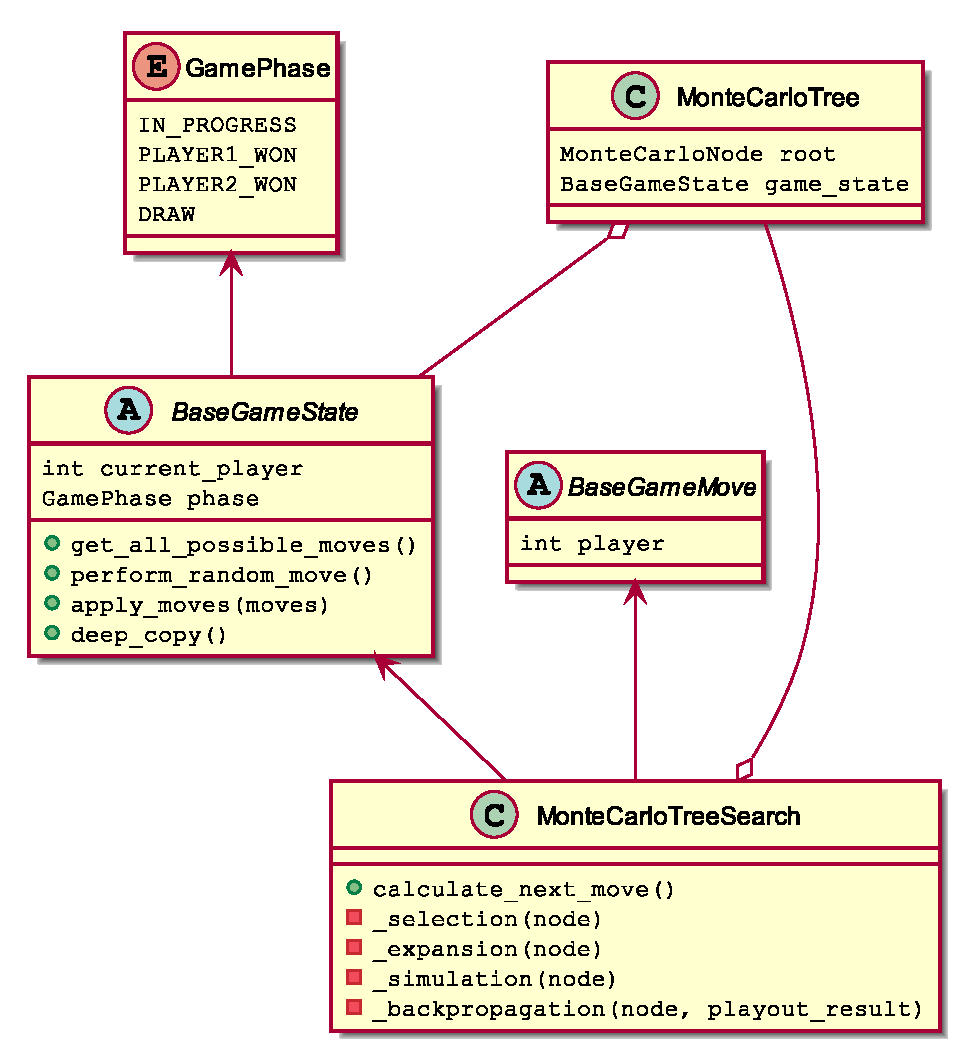
\includegraphics[width=0.5\linewidth]{umldiagram_algorithm}
	\caption{Diagram UML dla modułu \textit{Algorytm}}
	\label{rys:umldiagram_algorithm}
\end{figure}

Zgodnie z Rysunkami \ref{rys:umldiagram_algorithm} i \ref{rys:umldiagram_serialization_visualisation}, klasy \textit{MonteCarloTreeSearch}, \textit{ImprovedWalkersAlgorithm} oraz \textit{Serializator} są pośrednio lub bezpośrednie zależne od klasy \textit{MonteCarloNode}, opisującej wierzchołek w drzewie. Jest to część wspólna modułów \textit{Algorytm}, \textit{Wizualizacja} i \textit{Serializacja}.

\begin{figure}[h!]
	\centering
	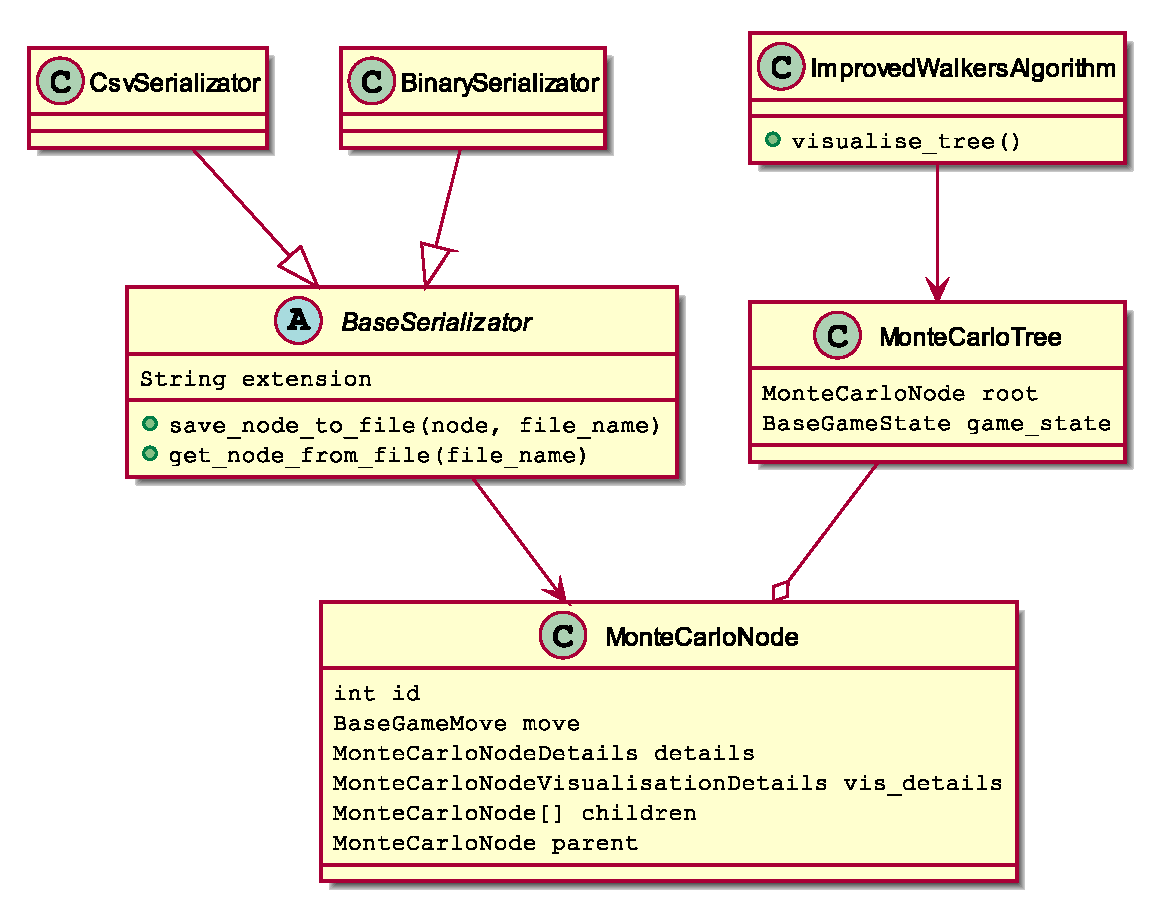
\includegraphics[width=0.6\linewidth]{umldiagram_serialization_visualisation}
	\caption{Diagram UML dla modułów \textit{Serializacja} i \textit{Wizualizacja}}
	\label{rys:umldiagram_serialization_visualisation}
\end{figure}

\textit{Serializator} jest klasą opisującą funkcjonalności, które mają udostępnić właściwe implementacje serializatorów, czyli serializowanie drzew do plików oraz deserializację z plików.

\section{Struktura stanów rozgrywki}
Rysunek \ref{rys:statediagram} ukazuje diagram stanów aplikacji w przypadku rozgrywki w trybie \textit{Gracz versus PC}. Zgodnie z diagramem, aplikacja po zainicjowaniu rozgrywki przechodzi do stanu \textit{Rozgrywka} zawierającego cztery stany wewnętrzne. Będąc w stanie \textit{Rozgrywka}, aplikacja może korzysta z modułów \textit{Algorytm} i \textit{Wizualizacja}, a także opcjonalnie z modułu \textit{Serializacja}.\\

\begin{figure}[h]
	\centering
	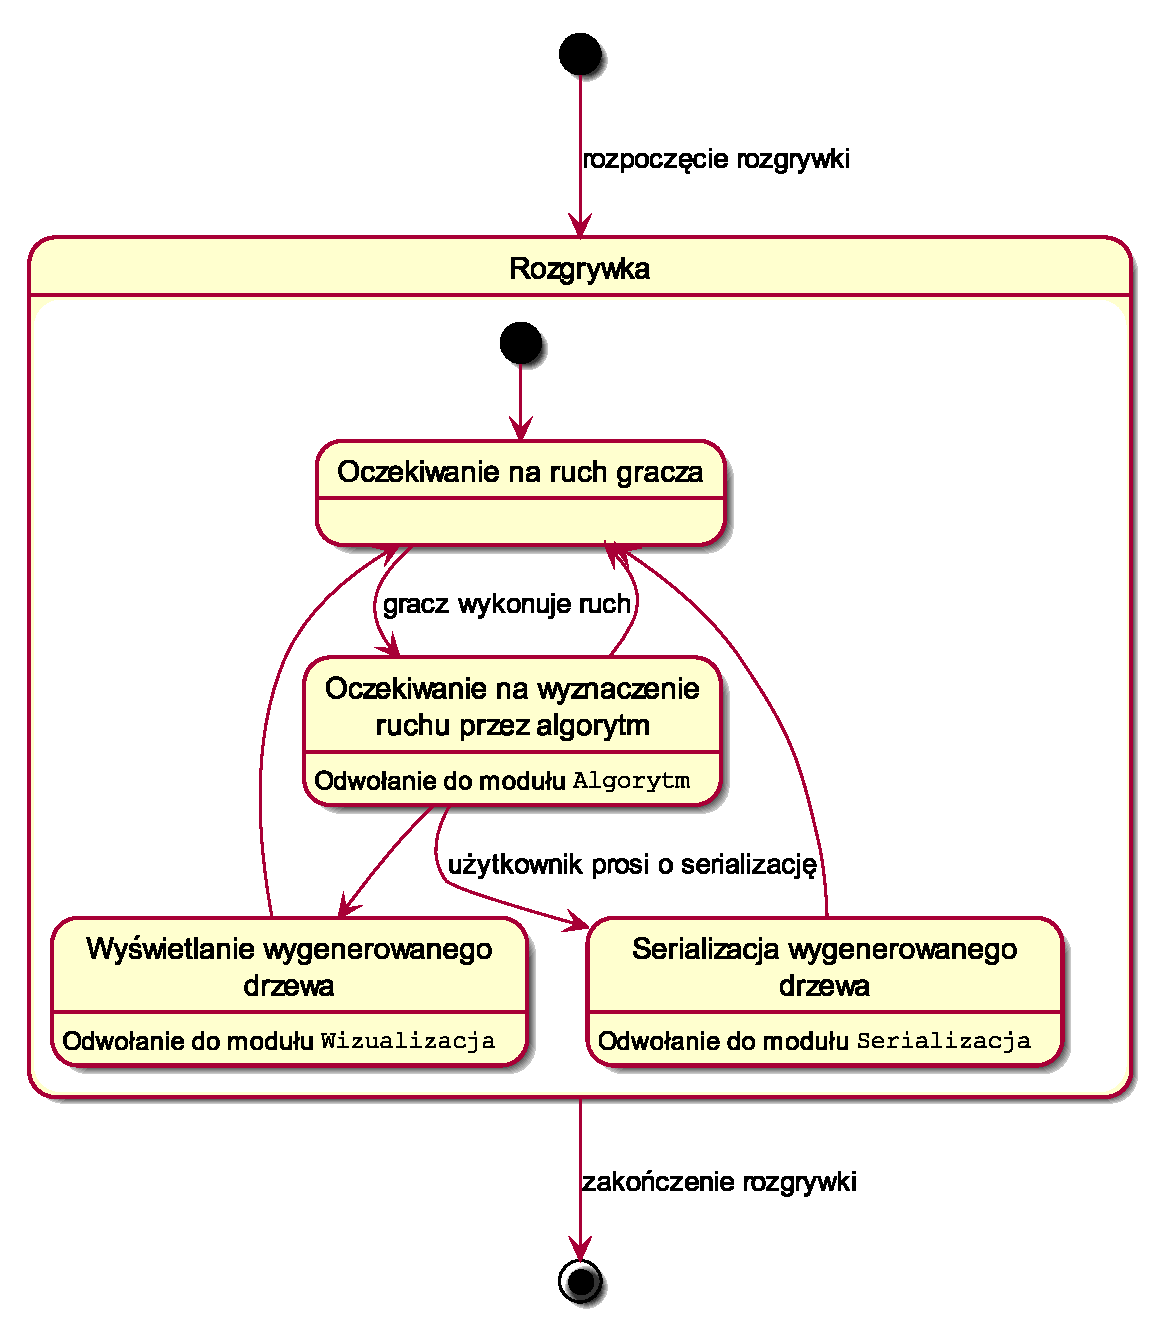
\includegraphics[width=0.7\textwidth]{state_diagram}
	\caption{Diagram stanów aplikacji}
	\label{rys:statediagram}
\end{figure}

Istotna z punktu widzenia użytkownika jest wizualizacja drzewa stanów bezpośrednio po ruchu wyznaczonym przez algorytm, co powoduje przejście aplikacji odpowiednio w stany \textit{Serializacja wygenerowanego drzewa} oraz \textit{Wyświetlanie wygenerowanego drzewa}, a także możliwość serializacji i zapisania powstałego drzewa -- stan \textit{Serializacja wygenerowanego drzewa}.

\section{Struktura sekwencji rozgrywki}
Rysunek \ref{rys:sequencegame} ukazuje diagram sekwencji rozgrywki w trybie \textit{Gracz versus PC}. Na diagramie przedstawiona jest istota komunikacji głównych modułów podczas rozgrywania partii w jedną z dwóch gier. \textit{Aplikacja główna}, \textit{Gra} i \textit{Algorytm}.\\

\begin{figure}[h]
	\centering
	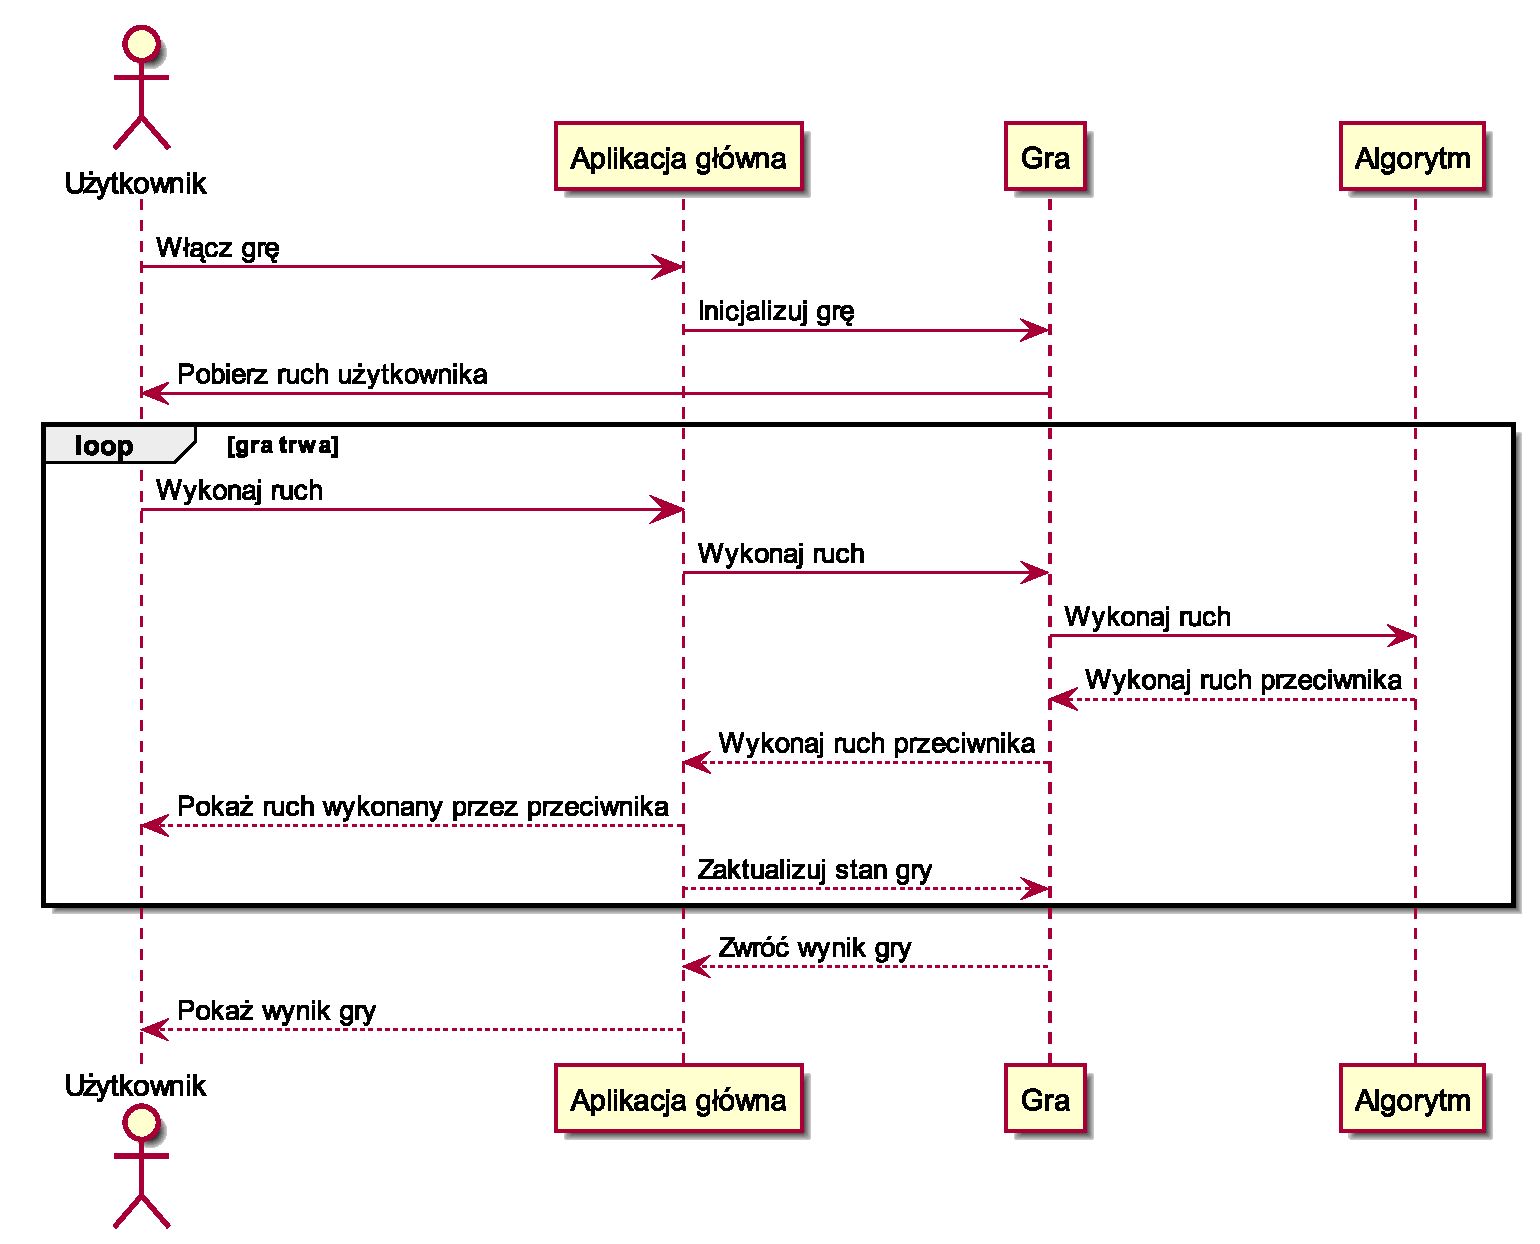
\includegraphics[width=1\textwidth]{play_with_pc_sequence}
	\caption{Diagram sekwencji rozgrywki}
	\label{rys:sequencegame}
\end{figure}

Użytkownik końcowy za pomocą menu aplikacji głównej może ustawić parametry gry i uruchomić ją. Inicjalizowana jest wówczas rozgrywka w komponencie \textit{Gra}. Następnie, dopóki gra trwa i możliwe jest wykonanie ruchu, wykonywane są na zmianę ruchy gracza i PC -- wymaga to komunikacji odpowiednio użytkownika z aplikacją główną, aplikacji głównej z grą i gry z modułem \textit{Algorytm} (i na odwrót). Po zakończeniu rozgrywki gra zwraca swój stan, który jest możliwy do zobaczenia przez użytkownika poprzez okno aplikacji głównej. Dodatkowo, po każdym wykonanym ruchu, za pomocą modułu \textit{Wizualizacja} generowane jest drzewo stanów algorytmu UCT, a następnie pokazywane jest ono użytkownikowi.\\

Diagram ukazuje, że w tym trybie każdy ruch gracza jest ściśle związany z odpowiedzią od modułu \textit{Algorytm}, który pobiera stan rozgrywki z modułu \textit{Gra}.


\section{Struktura sekwencji eksportu drzewa}
Rysunek \ref{rys:sequenceserialize} przedstawia proces współpracy różnych komponentów aplikacji w celu wyeksportowania wygenerowanego przez algorytm drzewa podczas rozgrywki. Proces uruchamiania gry i wykonywania ruchów jest analogiczny do tego na Rysunku \ref{rys:sequencegame}. 
\begin{figure}[h]
	\centering
	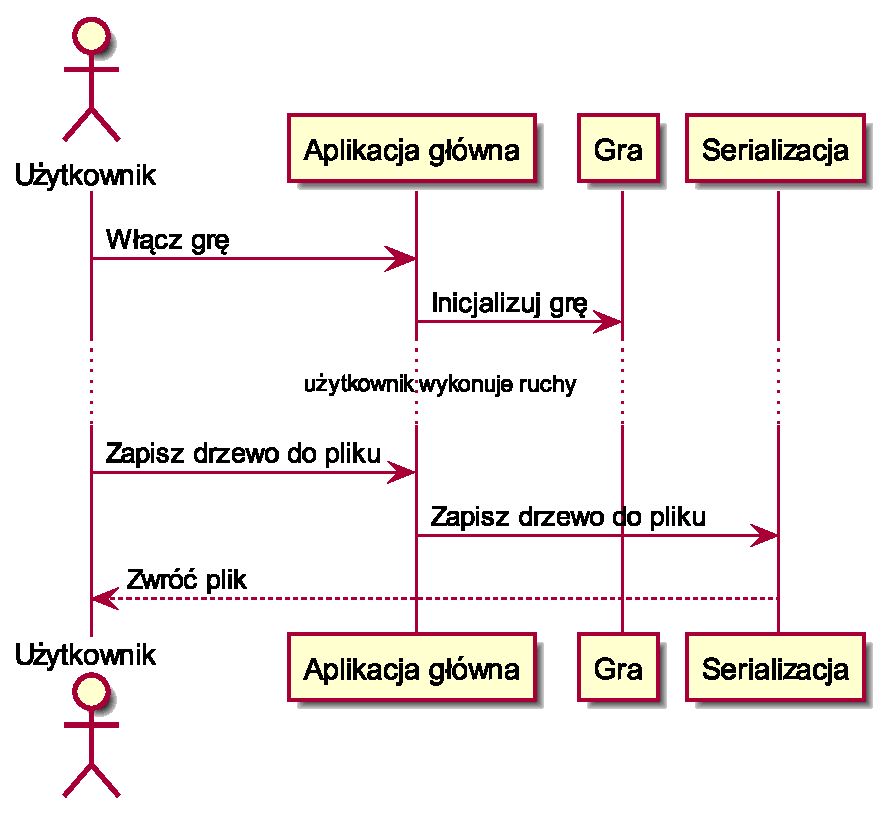
\includegraphics[width=0.7\textwidth]{serialize-seq}
	\caption{Diagram sekwencji eksportu drzewa}
	\label{rys:sequenceserialize}
\end{figure}

Istotną cechą zaprojektowanego rozwiązania jest to, że gracz może wyeksportować drzewo w dowolnym momencie rozgrywki (po każdym ruchu przeciwnika). Żądanie takiej operacji przez użytkownika przesyłane jest do aplikacji głównej, która następnie komunikuje się z modułem odpowiedzialnym za serializację, który zapisuje drzewo do pliku. Plik drzewa zapisywany jest do wybranego przez użytkownika folderu.\\

Jest to diagram dla trybu rozgrywki \textit{Gracz versus PC}, jednak w przypadku ustawienia \textit{PC versus PC} sposób serializacji się nie zmienia i diagram wygląda identycznie.

\section{Struktura sekwencji wizualizacji drzewa}
Rysunek \ref{rys:sequencevisualise} przedstawia proces wyświetlania wizualizacji drzewa przez użytkownika jako współpracę poszczególnych komponentów aplikacji. Ponownie, proces uruchamiania gry i wykonywania ruchów wygląda tak jak na Rysunku \ref{rys:sequencegame}.
\begin{figure}[h]
	\centering
	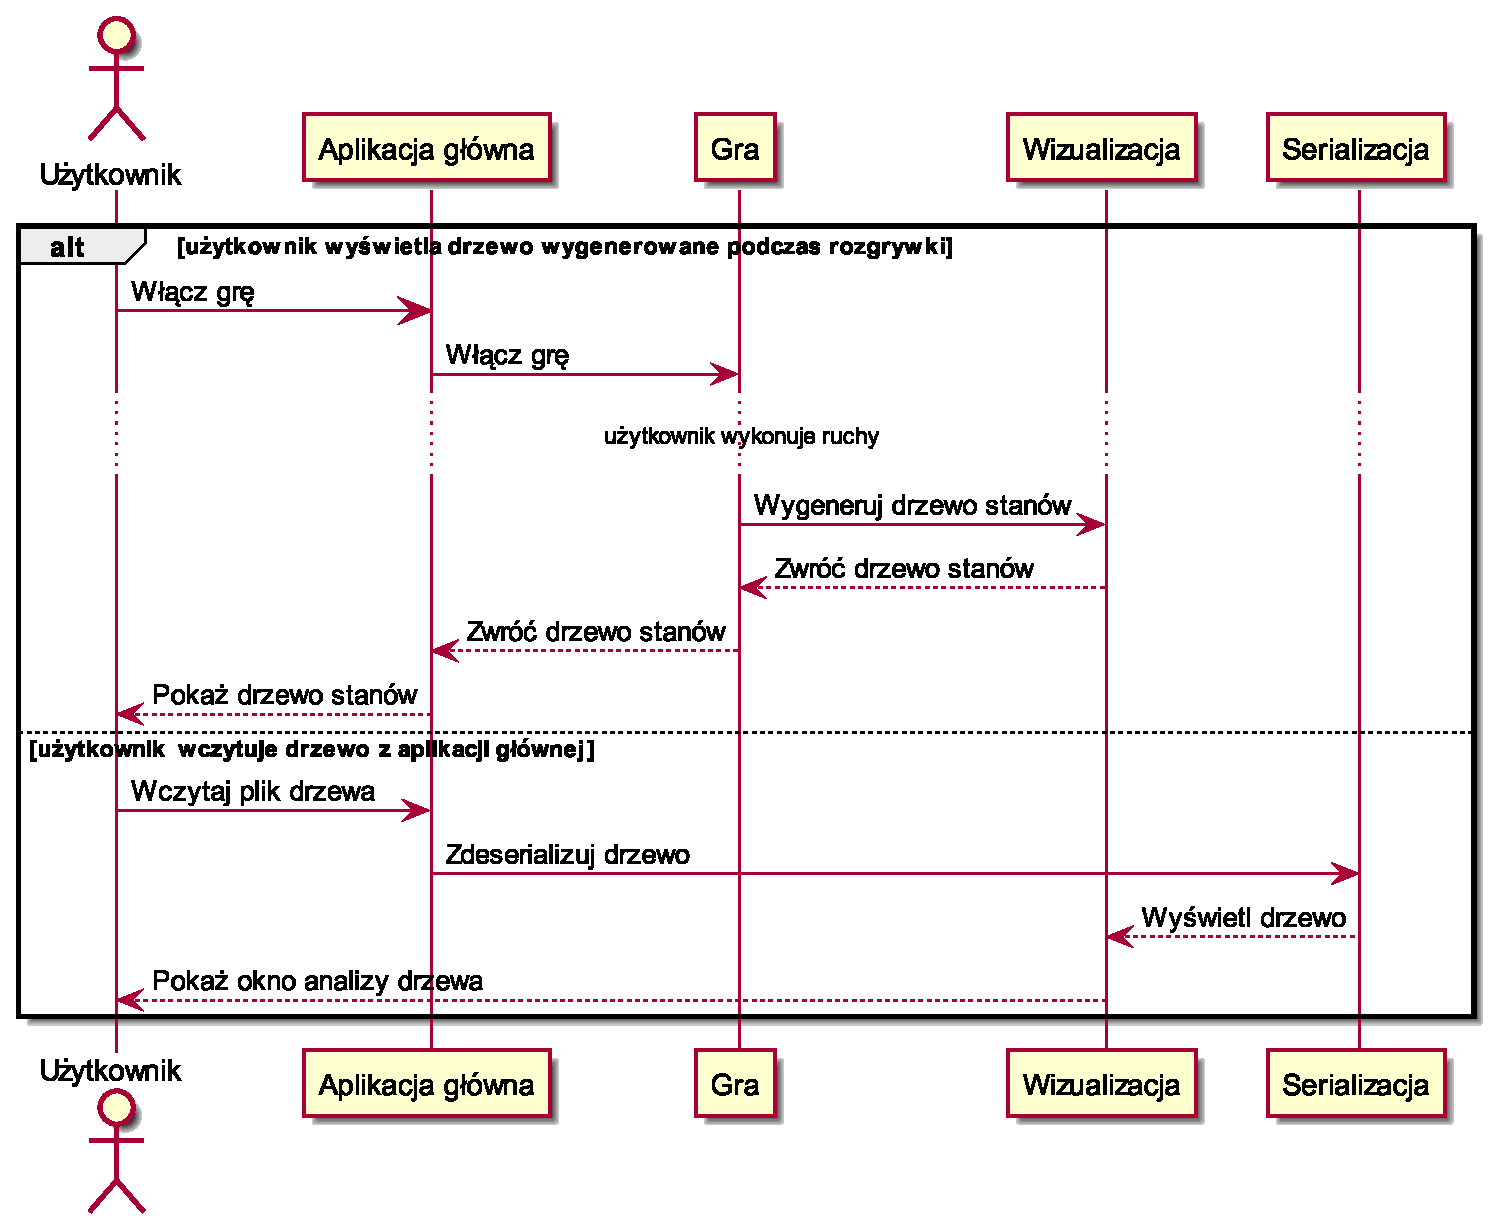
\includegraphics[width=1\textwidth]{visualisation-seq}
	\caption{Diagram sekwencji wizualizacji drzewa}
	\label{rys:sequencevisualise}
\end{figure}

Istotny jest fakt, że użytkownik może oglądać drzewa stanów wybierając pliki drzew z dysku w menu głównym aplikacji, ale też oglądać je bezpośrednio podczas rozgrywki po wykonanym ruchu algorytmu. Gdy żądanie jest z poziomu rozgrywki, komponent \textit{Aplikacja główna} komunikuje się z komponentem \textit{Wizualizacja}, który generuje aktualne drzewo i pokazuje je użytkownikowi na ekranie.\\

Drugi sposób, czyli wczytanie plików drzew z menu głównego, wymaga wcześniejszego zdeserializowania ich w celu wyświetlenia -- wymaga to komunikacji modułu \textit{Wizualizacja} i \textit{Serializacja}, gdzie ten drugi będzie zwracał wynik deserializacji temu pierwszemu. Następnie, analogicznie, użytkownik będzie mógł zobaczyć okno z wygenerowanymi drzewami.\\
